\clearpage
\chapter{Results}

\section{Test-bed Architecture}

The problem stated in Section~\ref{problem} was used to computationally test the topics discussed in this paper. In terms of test bed architecture, the timings were all conducted on a 3.4~Ghz Intel Core~i5-3570K. with 6~Mb cache and 4 cores along with 16~GB of DDR3 memory. For the GPU times, two cards were used: a Kepler architecture, Tesla~K40 clocking 745~Mhz-875~Mhz, carrying 15 SMs, each with 192 CUDA cores, it carries 12~GB of GDDR5 global memory clocking 1.5~GHz and a 288~GB/s bandwidth. The other card tested was the more modern, Turing architecture, RTX~2080 Super, clocking at 1.65~Ghz-1.815~Ghz, carrying 48 SMs, each with 64 CUDA cores, 8~GB of GDDR6 memory with a 496GB/s bandwidth. Both cards have 48~Kb of shared memory per block and 16~Kb of per thread memory available. Note also, due to the limitations of the most recent version of Nvidia's Visual Profiler tool, installed on the system mentioned, and also the removal of some of the counters from the Turing architecture, for profiling, a different system with an older version of NVVP and an older Kepler architecture GeForce GTX~780. The GTX~780 clocks at 869~Mhz-900~Mhz, has 2304 CUDA cores, and 3~GB of GDDR5 DRAM with 288~GB/s bandwidth. The system was also using an Intel Core~i5~7600 with 3.5~Ghz clock speed, 6 cores and 6~MB L3 cache. Table~\ref{table:testbed} illustrates all the specifications for the setup.
\begin{table}
    \begin{center}
    \resizebox{\columnwidth}{!}{
    \begin{tabular}{L{9em}|C{4em}C{5em}C{3em}C{6em}C{8em}C{5em}C{5em}@{}m{0pt}@{} }
        %\Xhline{3\arrayrulewidth}
        \hline
        GPU & Arch & Clock~Speed & SMs & CUDA~Cores & DRAM & Bandwidth & Shared &\\[1.5em]
        \hline
        Tesla~K40 & Kepler & 745~Mhz & 15 & 2880 & 12~GB~GDDR5 & 288~GB/s & 46~Kb &\\[1.35em]
        RTX~2080~Super & Turing & 1.65~Ghz & 48 & 3072 & 8~GB~GDDR6 & 496~GB/s & 46~Kb &\\[1.35em]
        GeForce~GTX~780 & Kepler & 869~Mhz & N/A & 2304 & 3~GB~GDDR5 & 288~GB/s & 46~Kb &\\[1.35em]
        %\Xhline{3\arrayrulewidth}
        \hline
    \end{tabular}}
    \caption{Testbed architecture.}
	\label{table:testbed}
	\end{center}
\end{table}
From a software perspective, all serial code was written in C++11 and compile using \texttt{gcc5.4.0} with \texttt{-O3} flag enabled. The \texttt{-std=c++11} flag was of course enabled to ensure that the correct version of C++ and the STL was being utilised. In order to take advantage of the linear solvers, the Intel's MKL 18.0.4 library also needed to be called compiled with the serial code. To enable this, the binary executable and library files needed to be appended to the \texttt{PATH} and \texttt{LD\_LIBRARY\_PATH} environment variables, this was done by either calling the correct modules, if available or manually appending by,
\begin{lstlisting}[style = bashStyle]
export PATH=$PATH:/home/support/apps/intel/18.0.4/bin/
export LD_LIBRARY_PATH=$LD_LIBRARY_PATH:/home/support/apps/intel/18.0.4/mkl/lib/intel64/intel64/
\end{lstlisting}
. The list of flags then needed for the Make were as follows,
\begin{itemize}
	\item \texttt{-lm}
	\item \texttt{-lmkl\_intel\_lp64}
	\item \texttt{-lmkl\_sequential}
	\item \texttt{-lmkl\_core}.
\end{itemize}

For the GPU code, all of it was written in CUDA with the most recent 10.1 SDK. The code was compiled with \texttt{nvcc} and \texttt{-O3} flag enabled again. In the implementation, certain device functions are shared across different headers so the \texttt{--relocatable-device-code=true} flag had to be enabled. the last consideration for the setup is the CUDA SDK~10.1, and its libraries used for linear solutions and BLAS operations. To enable these, again the \texttt{PATH} and \texttt{LD\_LIBRARY\_PATH} environment variables had to be appended, in this instance by,
\begin{lstlisting}[style = bashStyle]
export PATH=$PATH:/usr/local/cuda-10.1/bin
export LD_LIBRARY_PATH=$LD_LIBRARY_PATH:/usr/local/cuda-10.1/lib64
\end{lstlisting}
. The list of flags then needed:
\begin{itemize}
	\item \texttt{-lcusolver}
	\item \texttt{-lcusparse}
	\item \texttt{-lcublas}.
\end{itemize}

\begin{remark}
For all the testing mentioned in the rest of this chapter, each data point, or setup combination was run 5 times and the mean score taken. All models were plotted using \texttt{ggplot2} and loess smoothing fitted with linear, quadratic or logarithmic regression depending on the data. All grey ribbons represent 95\% confidence intervals for these models.
\end{remark}

\section{Serial Code Profiling}

\section{GPU Performance}

\subsection{Standard FEM}

The standard FEM GPU approach achieved some varying times depending largely on whether or not the choice of sparse or dense solves were used. The generation of the element matrices and assembly of the stiffness matrices reached some quite substantial speedups. However, as is detailed in this section, these kernel timings were dominated by the far more computationally expensive linear solvers.

\subsubsection{Total Timings}

\begin{figure}
	\centering
	\begin{subfigure}{0.48\linewidth}
		\centering
		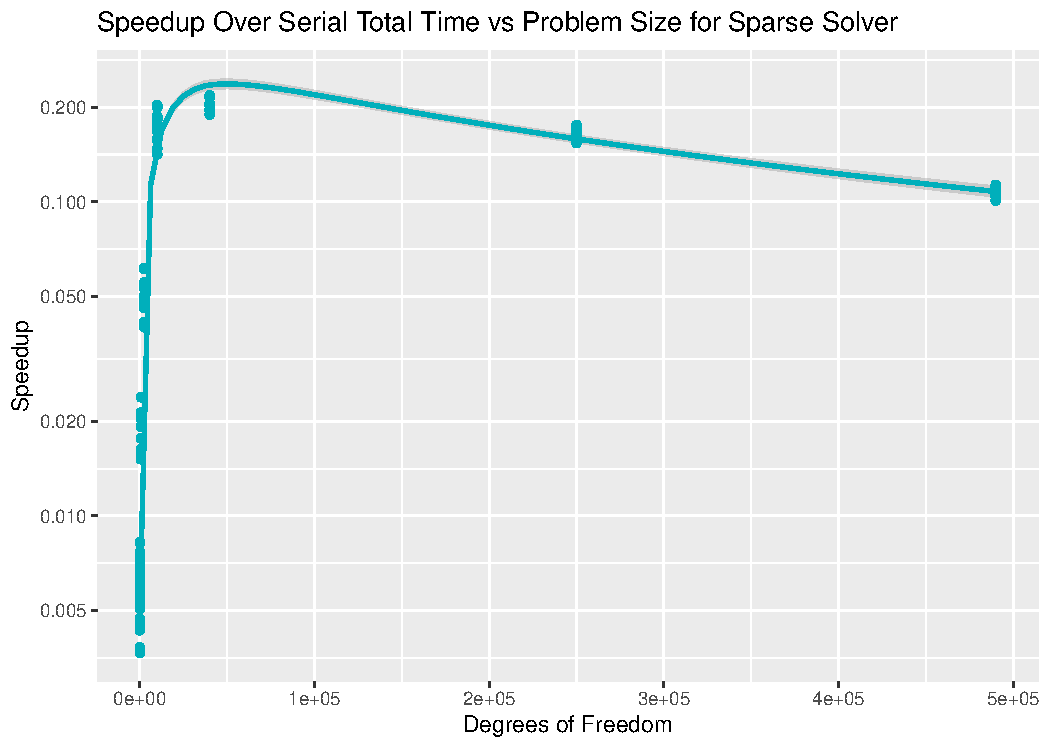
\includegraphics[width = \linewidth]{Plots/total_sparse_cpu_speedup_vs_n}
		\caption{Caption}
		\label{fig:tot_sparse}
	\end{subfigure}\hfill
	\begin{subfigure}{0.48\linewidth}
		\centering
		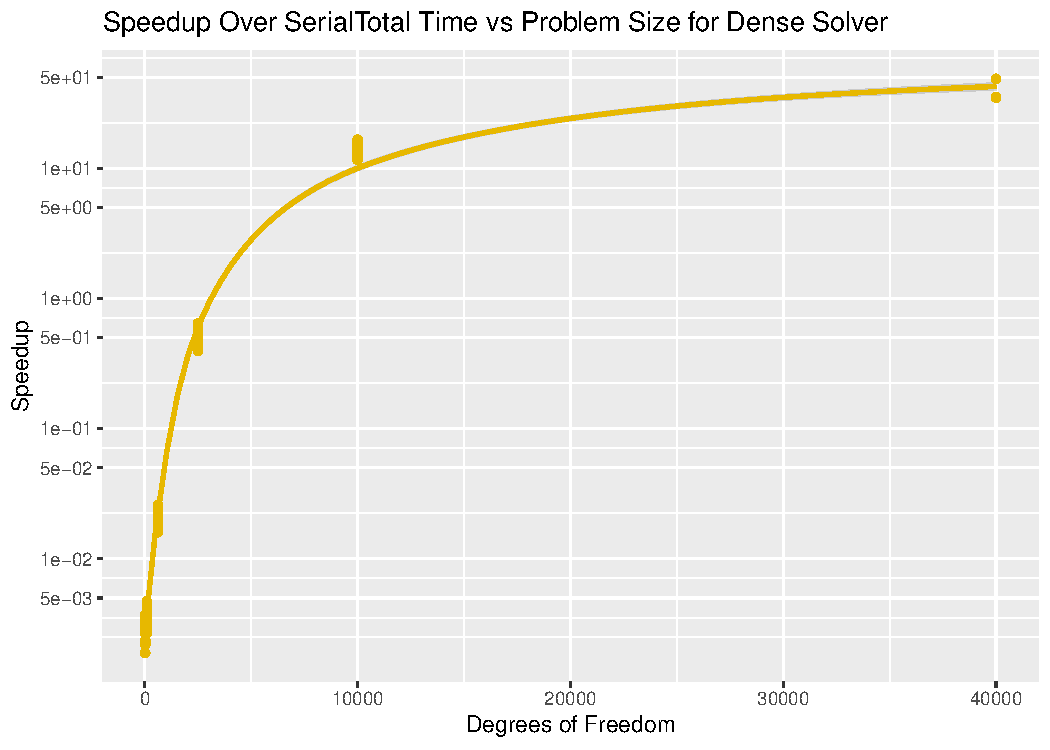
\includegraphics[width=\linewidth]{Plots/total_dense_cpu_speedup_vs_n}
		\caption{Caption}
		\label{fig:tot_dense}
	\end{subfigure}\\
	\begin{subfigure}{0.48\linewidth}
		\centering
		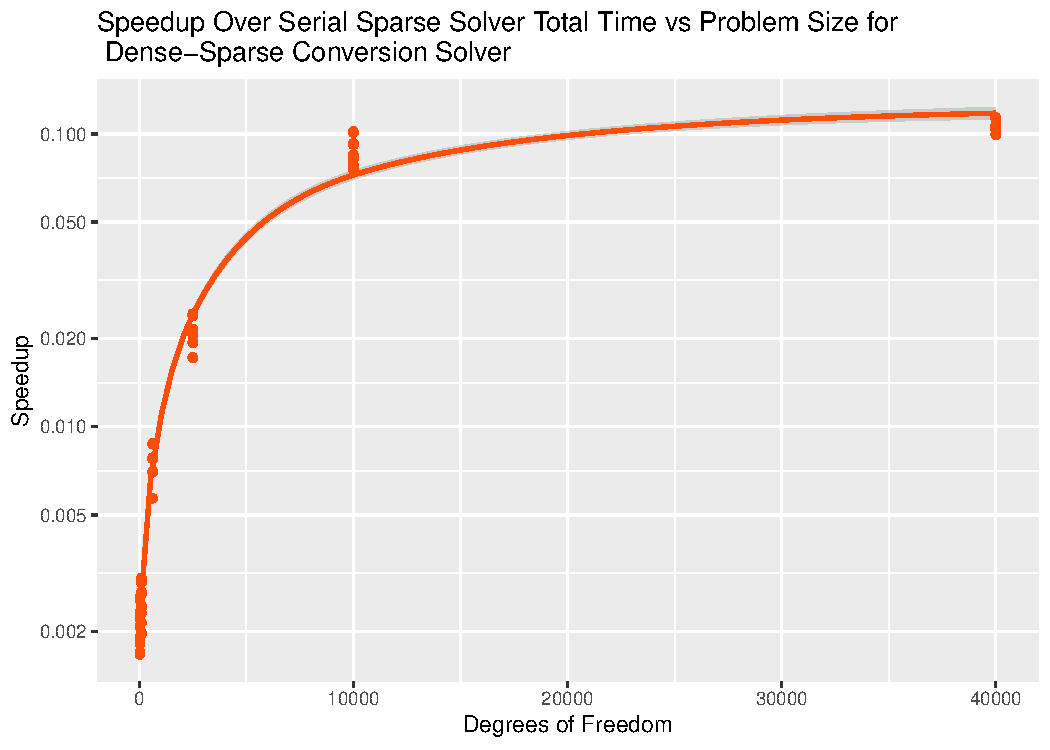
\includegraphics[width=\linewidth]{Plots/total_dnsspr_cpu_sparse_speedup_vs_n}
		\caption{Caption}
		\label{fig:tot_dnsspr_sparse}
	\end{subfigure}\hfill
	\begin{subfigure}{0.48\linewidth}
		\centering
		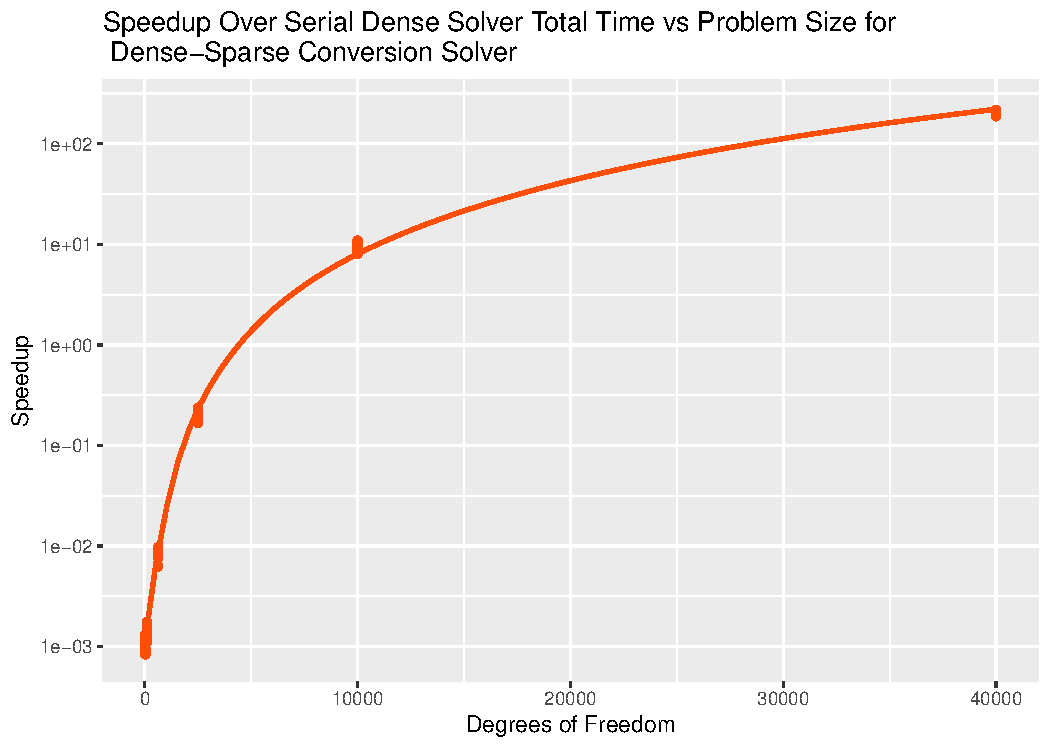
\includegraphics[width=\linewidth]{Plots/total_dnsspr_cpu_dense_speedup_vs_n}
		\caption{Caption}
		\label{fig:tot_dnsspr_dense}
	\end{subfigure}
	\caption{Speed-ups of total times over serial code vs. problem size for sparse, dense and dense-sparse conversion solutions.}
	\label{fig:tot}
\end{figure}

Figure~\ref{fig:tot} illustrates the speed-ups of the total timings taken to complete the FEM for the various solver approaches against the problem size. Looking initially at the sparse or CSR variant, Figure~\ref{fig:tot_sparse} shows the speed-up over the sparse serial case. Clearly it does not actually achieve a speed-up at all but is in fact slower in all problem sizes. It does demonstrate and initial spike, but this can be written down to simply a factor of GPU programming. Often, for small problem sizes, there is an initial costs of transferring data from host to device, allocating memory on the device's DRAM and even just the card needing to "warm-up" - for lack of a better term.  For small problem sizes, this cost is proportionally much larger, and clearly as the number of unknowns grows, this factors in less. There is also, naturally much less parallelisation achievable at smaller problem sizes than larger ones. Thus, this spike is natural and to be expected and not really a result to be concerned about. What is more concerning was the lack of positive scaling. As it turns out, the total time is quite substantially dominated by the cuSOLVER sparse direct solver which happens to not perform anywhere near as optimally as Intel's DSS and even sees a decreasing scaling as problem size gets larger - though there is little can be done about that unfortunately.

The dense solver from a glance at Figure~\ref{fig:tot_dense}, demonstrates far more promising results. There is a clear logarithmic scaling there present in the graph. While clearly, again from the offset with small problem sizes, parallelising the problem is near not worth it and results in slower times. However, quite evidently, this improves quite rapidly and as the degrees of freedom approach 40000, the solver outperforms the serial code by a speedup of around $50\times$. Again here there is a substantial proportion of the computation time taken up by the linear solver which is shown later.

The dense-sparse conversion was compared to both the serial CSR solver and the serial dense solver in Figures~\ref{fig:tot_dnsspr_sparse}~\ref{fig:tot_dnsspr_dense}, since it sits somewhere in between both, having a dense assembly and sparse solver. Given that it was mentioned the proportion of computation time is considerable, it is to be expected that the dense-sparse solver performs poorly also by comparison to Intel's DSS - which it indeed does. The scaling has the same spike as the sparse-sparse comparison, though it is not immediately obvious due to the memory limitations of allocation larger problem sizes - which the pure CSR solve had the benefit of avoiding to a larger extent. This solver way out performs the purely dense serial solution, achieving massive speedups of up to $100\times$.

Figure~\ref{fig:tot_b} shows the speed-ups seen over the CPU code for sparse and dense solutions versus the choice of block size input from the command line. Without yet going into the details of the linear solvers computational dominance, in both cases, the stability in timings with variation of block size should tell enough that the purpose written code has little actual impact on the resulting final timings here. A benefit of the linear solvers is that they are optimised such that the best choice of block size to reduce warp divergence and maximise shared memory usage is selected for the user. Thus, meaning the choice of block size here should have not much impact - shown very much so below. Rather interestingly though, it does show the nice scaling with problem size for the dense case in Figure~\ref{fig:tot_dense_b} and the decreasing scaling for the sparse case in Figure~\ref{fig:tot_sparse_b}.
\begin{figure}
	\centering
	\begin{subfigure}{0.48\linewidth}
		\centering
		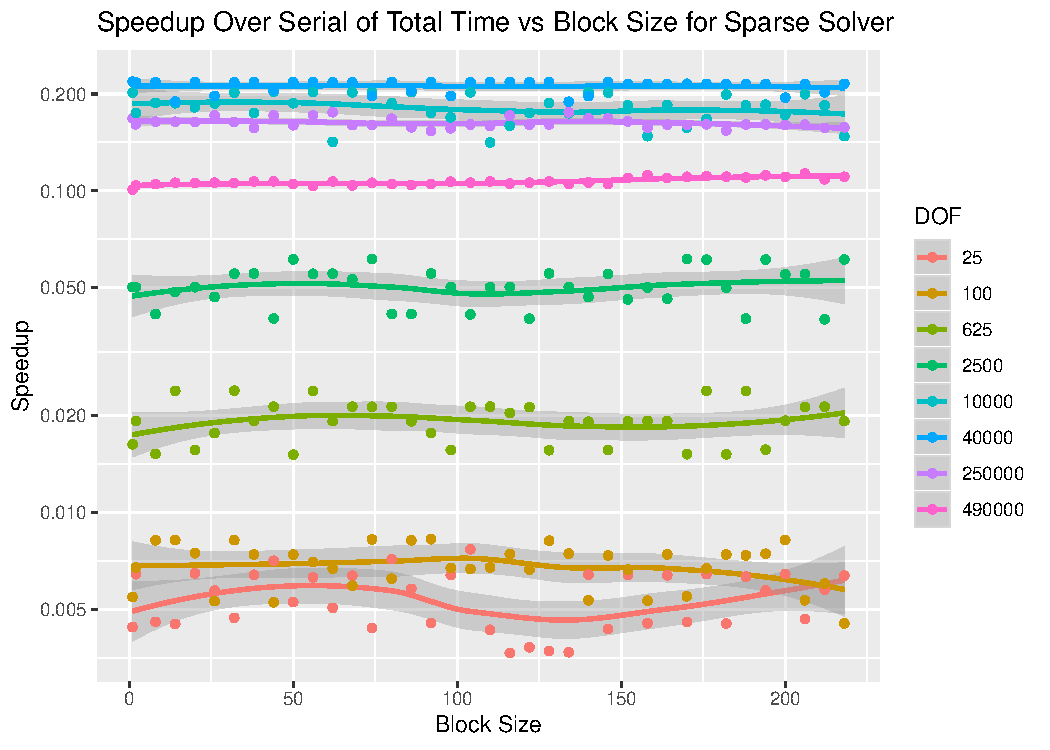
\includegraphics[width = \linewidth]{Plots/total_sparse_cpu_speedup_vs_b}
		\caption{Caption}
		\label{fig:tot_sparse_b}
	\end{subfigure}\hfill
	\begin{subfigure}{0.48\linewidth}
		\centering
		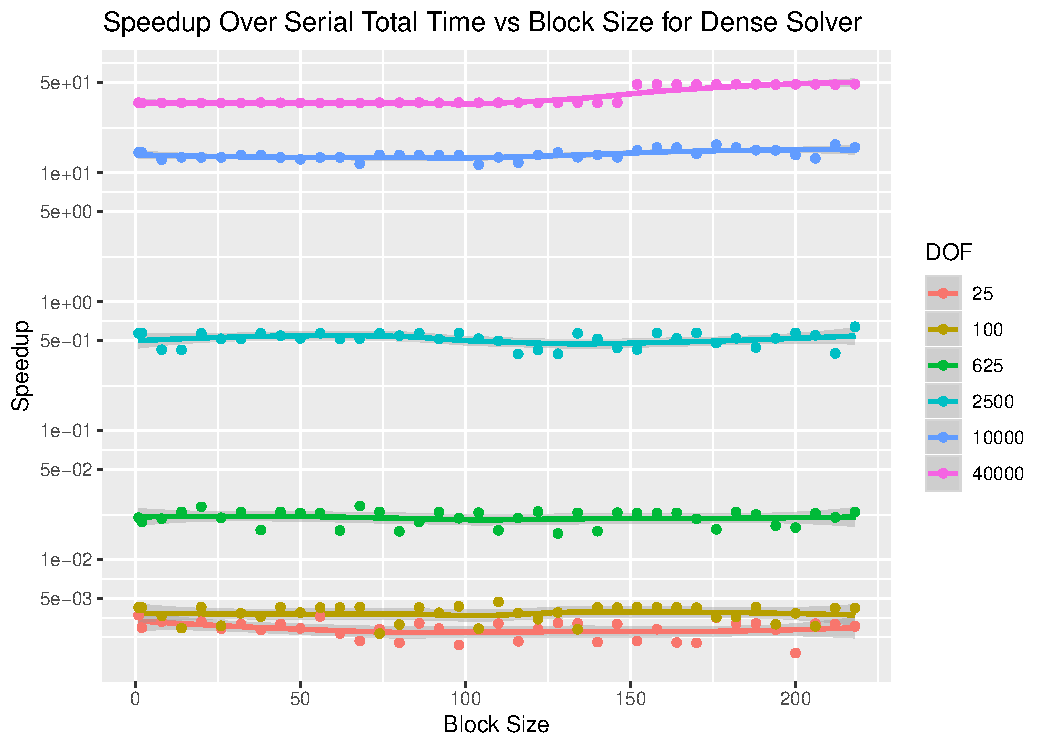
\includegraphics[width=\linewidth]{Plots/total_dense_cpu_speedup_vs_b}
		\caption{Caption}
		\label{fig:tot_dense_b}
	\end{subfigure}
	\caption{Speed-ups of total times over serial code vs. block size, for sparse \& dense solutions.}
	\label{fig:tot_b}
\end{figure}

\subsubsection{Linear Solvers}

\begin{figure}
	\centering
	\begin{subfigure}{0.48\linewidth}
		\centering
		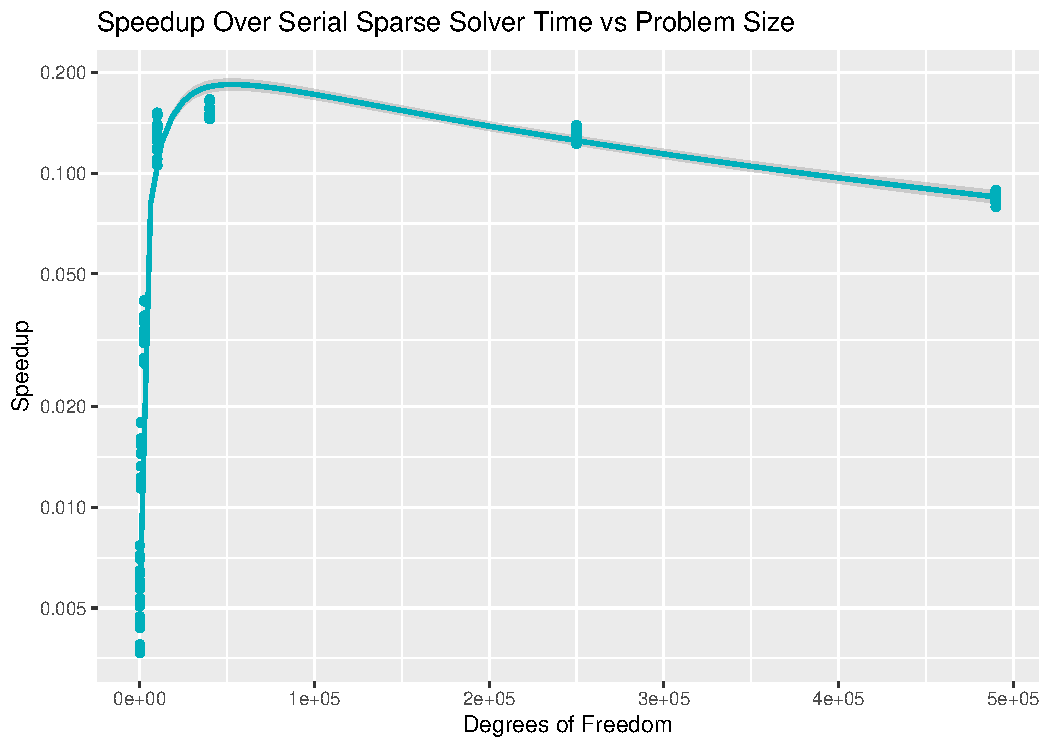
\includegraphics[width = \linewidth]{Plots/solve_sparse_cpu_speedup_vs_n}
		\caption{Caption}
		\label{fig:sparse_solver}
	\end{subfigure}\hfill
	\begin{subfigure}{0.48\linewidth}
		\centering
		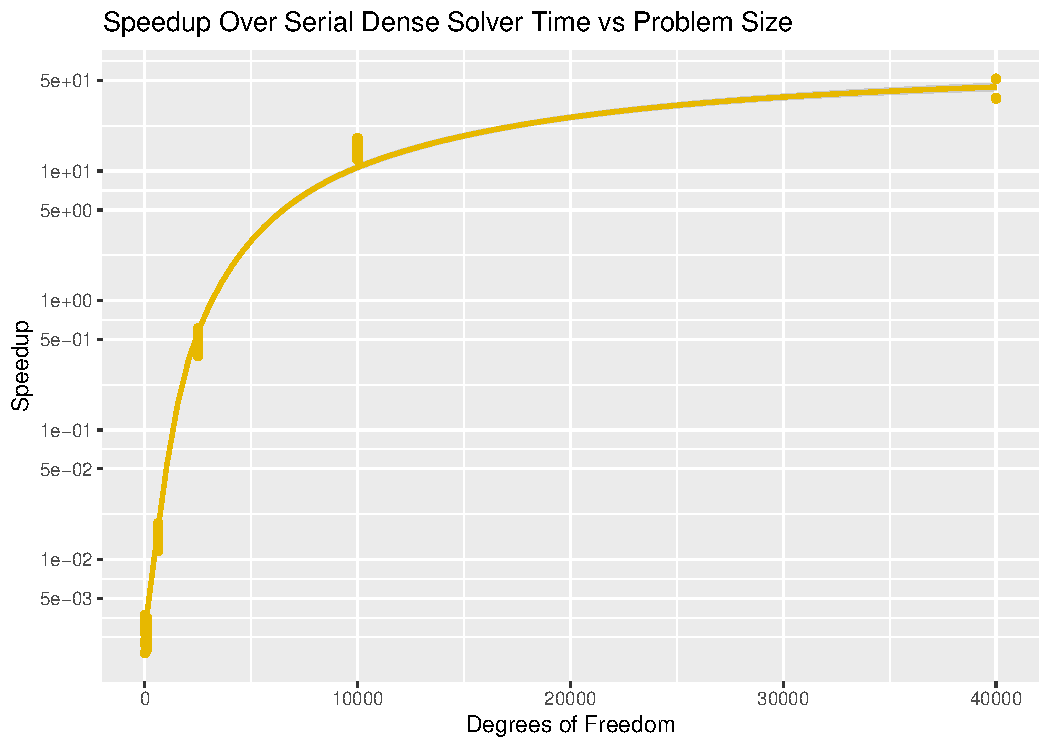
\includegraphics[width=\linewidth]{Plots/solve_dense_cpu_speedup_vs_n}
		\caption{Caption}
		\label{fig:dense_solver}
	\end{subfigure}
	\caption{Speed-ups of linear solver times over Intel's MKL vs. problem size, for sparse \& dense solutions.}
	\label{fig:solvers}
\end{figure}
Looking now at the actual performance of the linear solvers themselves. Figures~\ref{fig:sparse_solver},~\ref{fig:dense_solver} almost identically replicate the results seen in Figures~\ref{fig:tot_sparse},~\ref{fig:tot_dense} - just more illustrating how dominant these are towards the total time taken. In Figure (REFERENCE), this can be seen in screenshots taken from Nvidia's Visual Profiler the massive chunk of computation time taken by these solvers compared to the rest the FEM process. It isn't that these wholly perform poorly, more-so that Intel's DSS solve for CSR linear systems is optimised to very impressive levels, and simply outperforms Nvidia's cuSOLVER and cuSPARSE solutions. The dense solver on the other hand actually performs quite well compared to Intel's MKL library. It was not the premise of this paper to improve on existing direct linear solvers so this is simply a result that needs to be taken with a pinch of salt.

While it may seem that Nvidia's CSR solver is actually a poorly written and poorly performing piece of software, and one would be better off using the dense solver - this is certainly not the case, it just happens to not be as optimised as Intel's. Figure~\ref{fig:gpu_solve} illustrates the speed-ups seen of the sparse solver versus the dense solver as problem size increases. Clearly here, it gets up to around $10\times$ faster and is in fact a better performing solution than assembling a dense system and solving that. This is the benefits mentioned in Section~\ref{sparse} clearly in action.

\begin{figure}
	\centering
	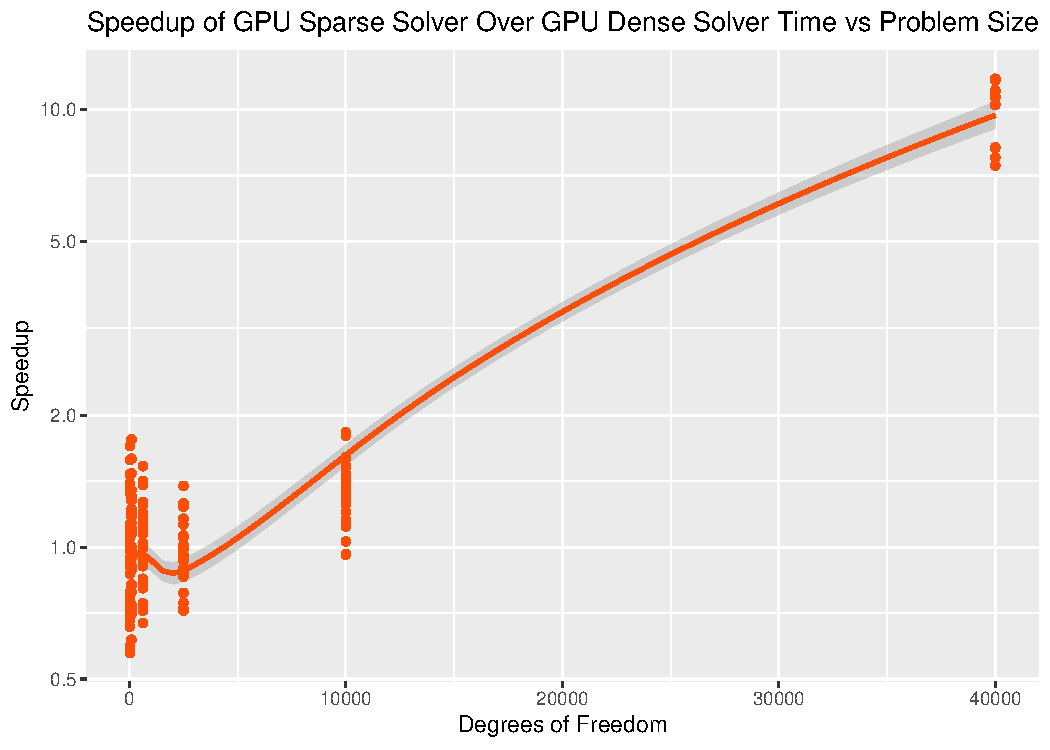
\includegraphics[width = 0.48\linewidth]{Plots/solve_gpus_speedup_vs_n}
	\caption{Speed-ups of Nvidia's sparse linear solver over their dense solver against problem size.}
	\label{fig:gpu_solve}
\end{figure}

\subsubsection{Allocation \& Transfer Times}

\begin{figure}
	\centering
	\begin{subfigure}{0.48\linewidth}
		\centering
		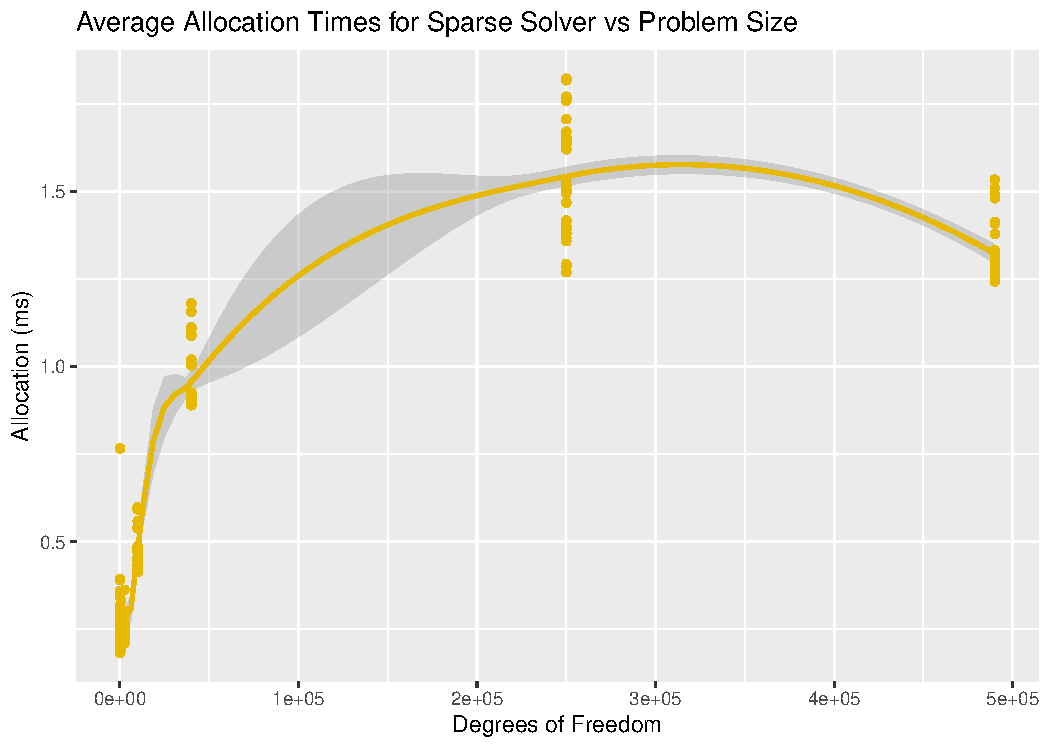
\includegraphics[width = \linewidth]{Plots/alloc_sparse_vs_n}
		\caption{Caption}
		\label{fig:alloc_sparse}
	\end{subfigure}\hfill
	\begin{subfigure}{0.48\linewidth}
		\centering
		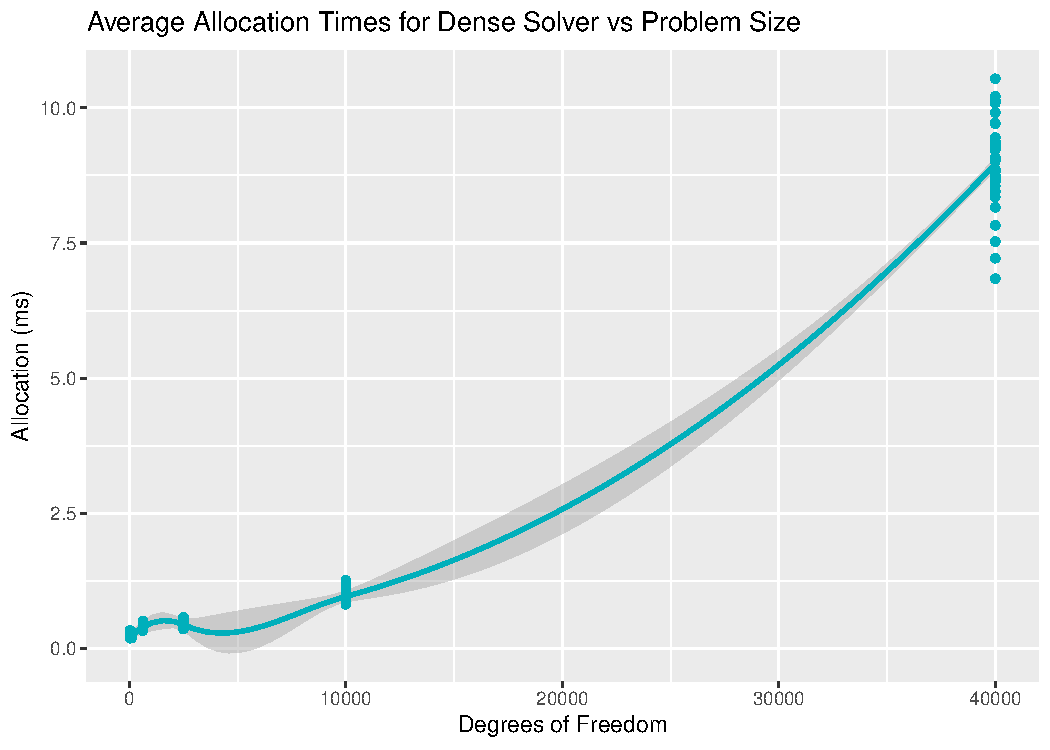
\includegraphics[width=\linewidth]{Plots/alloc_dense_vs_n}
		\caption{Caption}
		\label{fig:alloc_dense}
	\end{subfigure}
	\caption{Total allocation time taken for both dense and CSR approaches.}
	\label{fig:alloc}
\end{figure}
Figure~\ref{fig:alloc} shows the total allocation times for both sparse and dense cases. The dense case seen in Figure~\ref{fig:alloc_dense}, is not expected to have a linear scaling but more so a polynomial scaling. It illustrates a 2\textsuperscript{nd} order polynomial scaling, this is to be expected since, excluding the mesh, the dominant array needing to be allocated is of size $\texttt{order}\times{order}$. The sparse case, in Figure~\ref{fig:alloc_sparse}, on the other hand, is harder to predict the scaling of. This is due to the fact that as the matrix gets larger, the number of non-zeros present in the matrix will be totally dependent on the both the shape of the mesh as well as the degree of freedom ordering chosen for the model - be it P1 or P2 et cetera. The timing does appear to decrease, though the inclination here is that it is due to variance and the small sample size of 4 per data point - in this case four runs per block size and problem size. Figure~\ref{fig:alloc_su} shows the speed-up seen in performing the sparse case over the dense. Since both variants allocate the five arrays needed for the mesh as well as the stiffness matrix, naturally the expected, and observed, result here is sparse speed-up over dense.
\begin{figure}
	\centering
	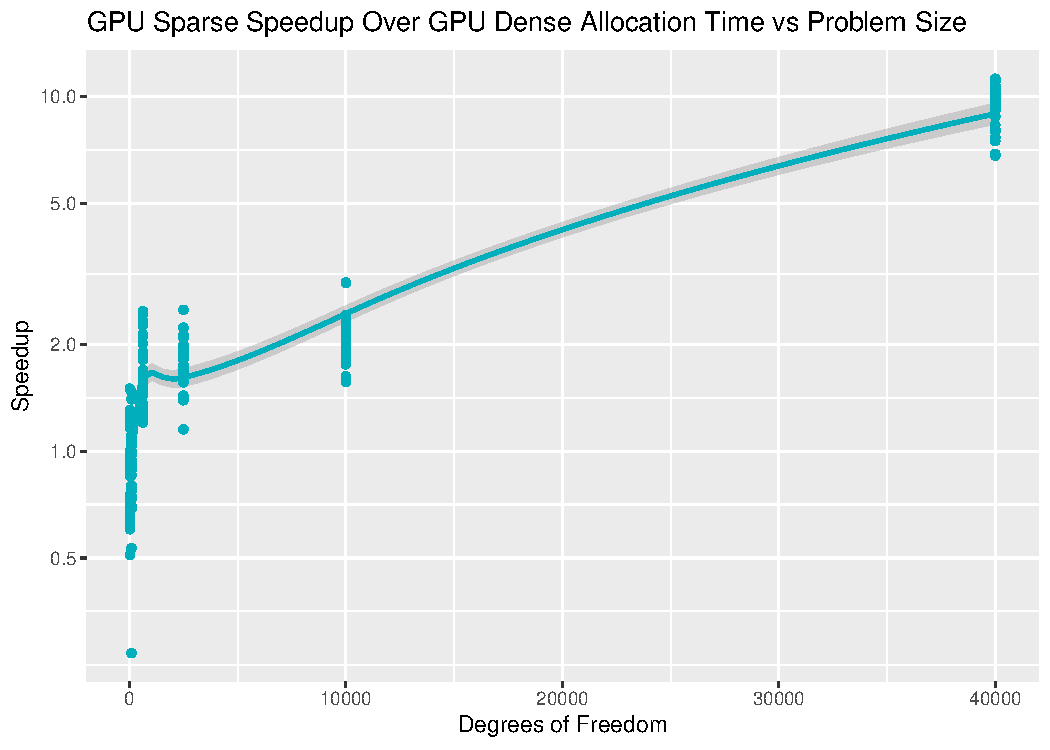
\includegraphics[width=0.48\linewidth]{Plots/alloc_sparse_dense_speedup_vs_n}
	\caption{Speed-up of allocation time taken for sparse case over dense versus problem size}
	\label{fig:alloc_su}
\end{figure}

\begin{figure}
	\centering
	\begin{subfigure}{0.48\linewidth}
		\centering
		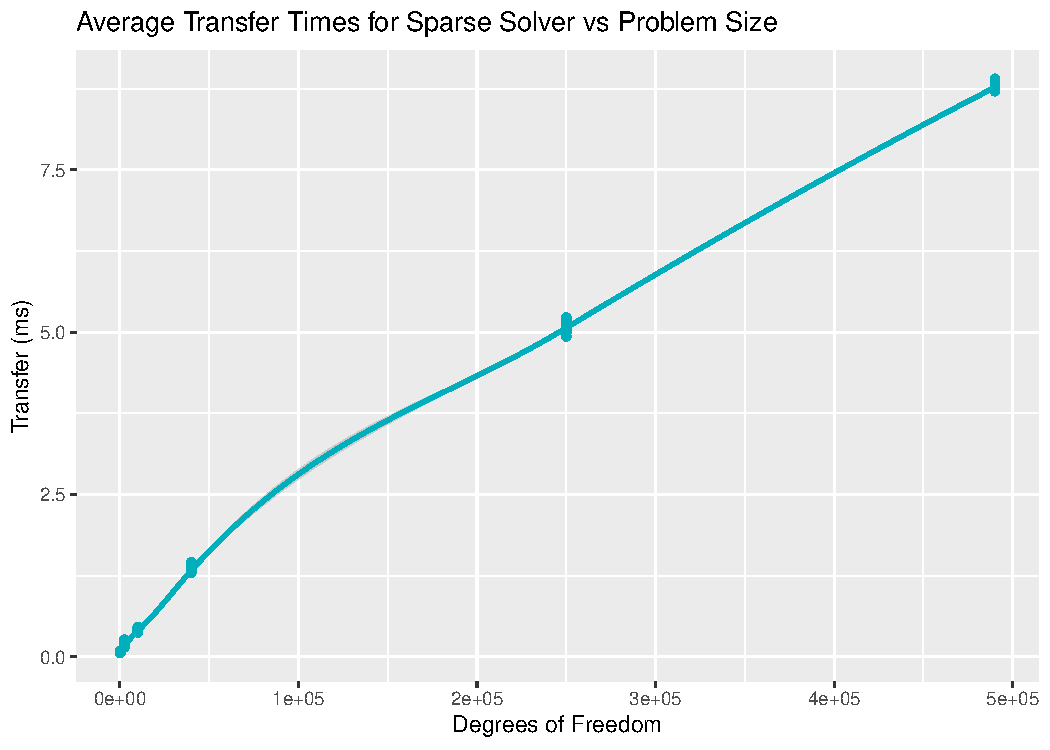
\includegraphics[width = \linewidth]{Plots/transf_sparse_vs_n}
		\caption{Caption}
		\label{fig:transf_sparse}
	\end{subfigure}\hfill
	\begin{subfigure}{0.48\linewidth}
		\centering
		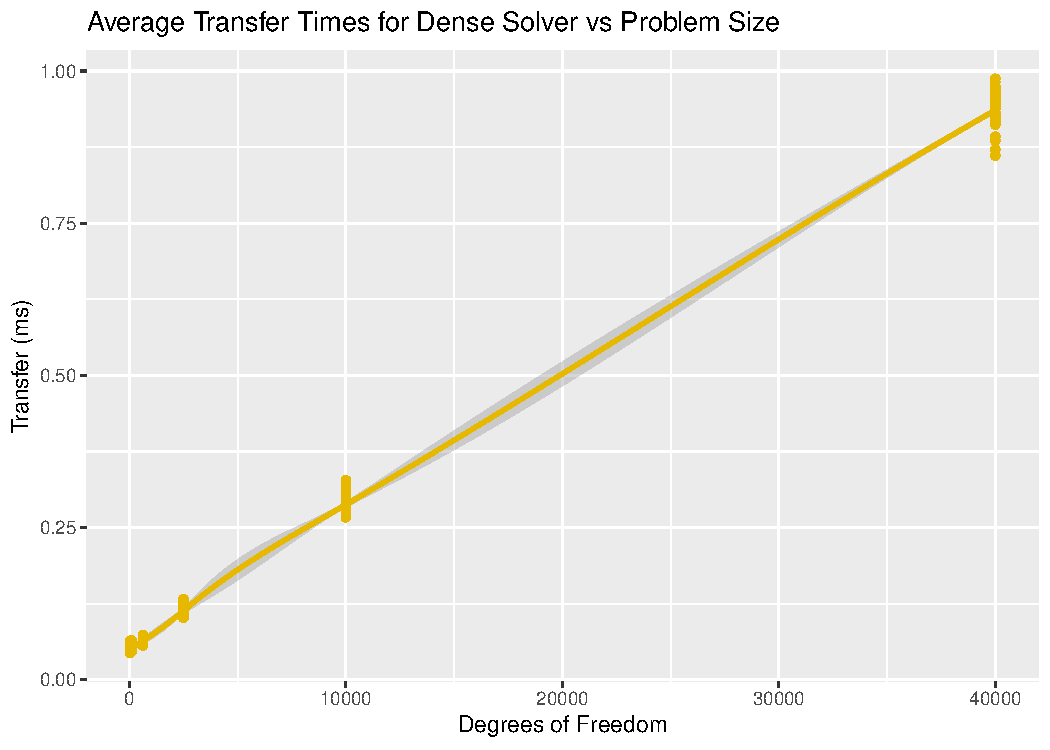
\includegraphics[width=\linewidth]{Plots/transf_dense_vs_n}
		\caption{Caption}
		\label{fig:transf_dense}
	\end{subfigure}
	\caption{Total transfer time taken for both dense and CSR approaches.}
	\label{fig:transf}
\end{figure}

Unlike in the allocation case, the sparse timings can be a bit more predictable. In the case of the allocations, all three of the arrays for the stiffness matrix had to be allocated, as well as the array for the stress vector. For the transfer, the mesh of course, as in allocation, needed to be transferred, the solution vector or former stress vector, but only two of the three CSR arrays. This should give rise to a much more linear scaling, as demonstrated in Figure~\ref{fig:transf_sparse}. It is not a perfect linear scaling, nor should it be, but the reduced effect of the irregularity of the CSR matrix is definitely evident. The dense case on the other hand, only transfers the mesh and the stiffness matrix, all of which scale in size linearly and thus, as is seen in Figure~\ref{fig:transf_dense}, observed a nice linear scaling. Figure~\ref{fig:transf_su} shows the speed-up seen in the sparse case over the dense. In this case, as would be entirely presumed, the dense case takes about 70\% of the time. Of course this would be expected given there is no sparsity pattern to transfer from the host. PUT IN TRANSFER BANDWIDTH?? 
\begin{figure}
	\centering
	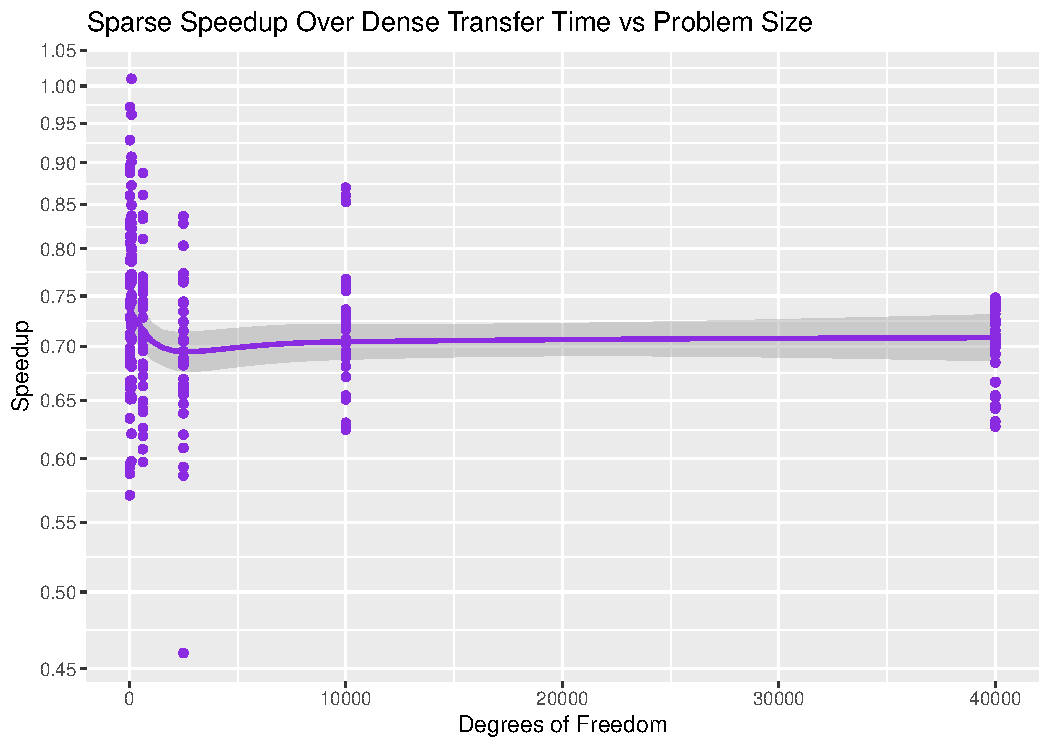
\includegraphics[width = 0.48\linewidth]{Plots/transf_sparse_dense_speedup_vs_n}
	\caption{Speed-up of transfer time needed for sparse over dense case versus problem size.}
	\label{fig:transf_su}
\end{figure}

\subsubsection{Element Matrices \& Vectors}

\begin{figure}
	\centering
	\begin{subfigure}{0.48\linewidth}
		\centering
		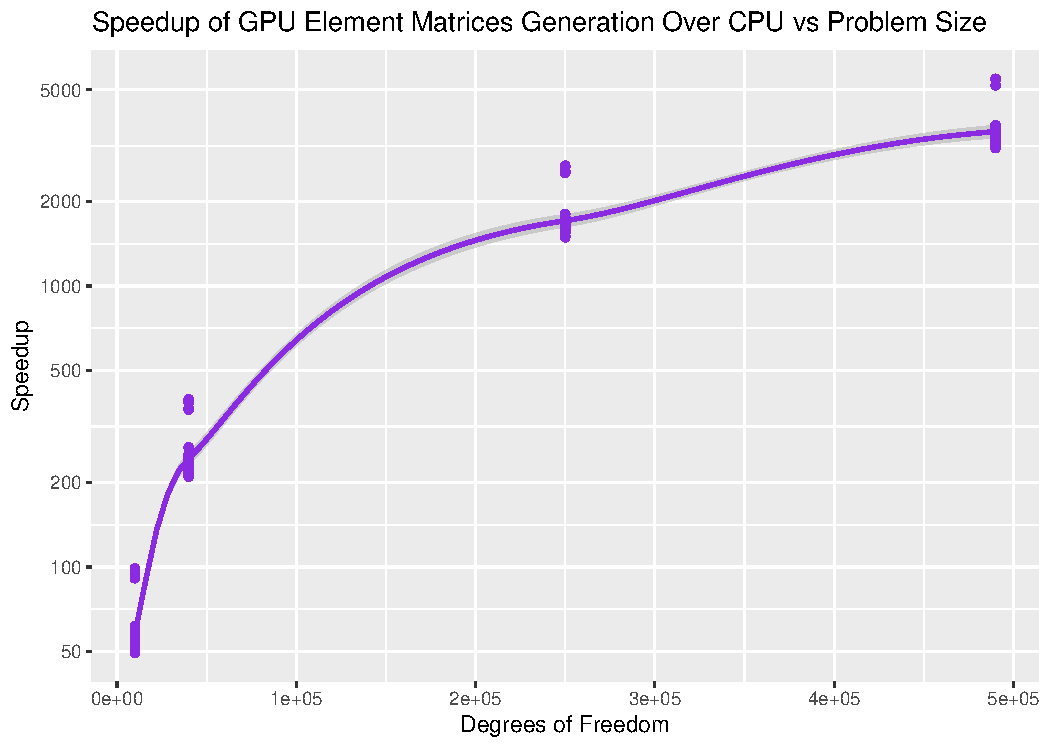
\includegraphics[width = \linewidth]{Plots/elem_mats_dev_cpu_speedup_vs_n}
		\caption{Caption}
		\label{fig:elems_n}
	\end{subfigure}\hfill
	\begin{subfigure}{0.48\linewidth}
		\centering
		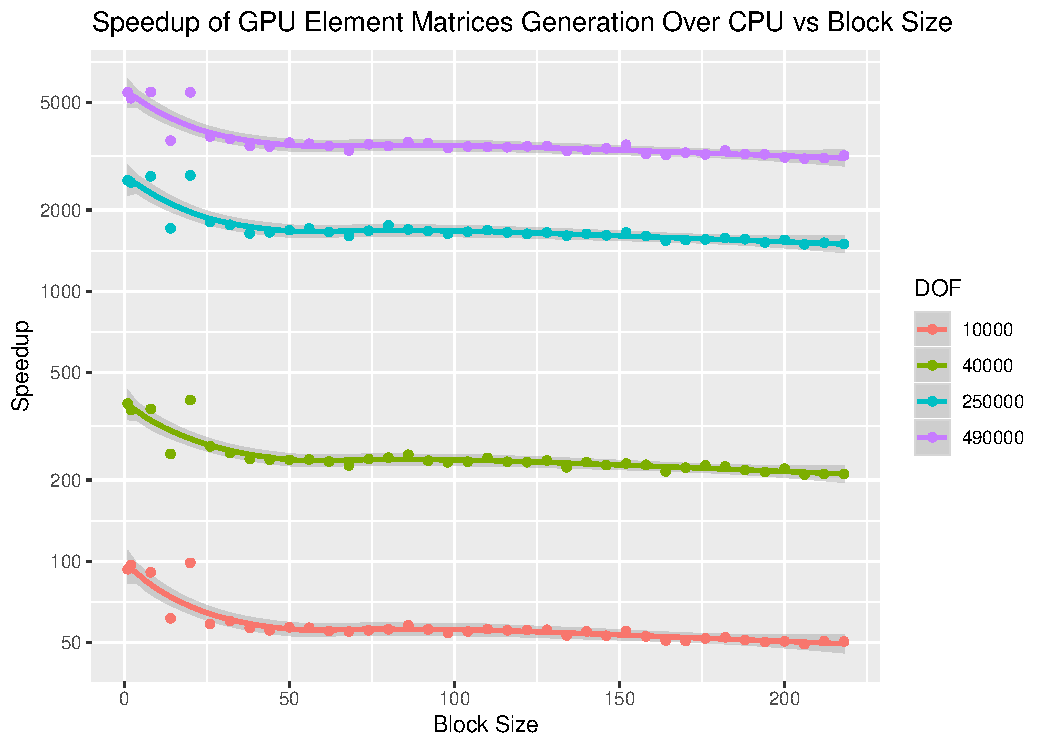
\includegraphics[width=\linewidth]{Plots/elem_mats_dev_cpu_speedup_vs_b}
		\caption{Caption}
		\label{fig:elems_b}
	\end{subfigure}
	\caption{Speed-ups of GPU generation of element matrices \& vectors over serial code against problem size \& block size.}
	\label{fig:elem_mats_gen}
\end{figure}

One of the two most relevant timings in this section is the generation of element matrices. As was discussed, there is a limited amount can be done about pre-existing linear solvers. However, there is a great deal of parallelism can be achieved when generating the element matrices and element vectors for the FEM. This is one of two of the the areas within which most of the though regarding optimisation was put. All the considerations mentioned in Section~\ref{gpu_model} were taken into account here: optimising shared memory and registry usage, minimisation of thread divergence from warps, coalescing memory when at all possible et cetera.

Figure~\ref{fig:elem_mats_gen} shows the massive speedups seen over the CPU against both problem size and block size when the device function was measured. There is a massive logarithmic scaling as the degrees of freedom increases, reaching up to $5000\times$ faster than the serial code for the largest problem size tested. In terms of the comparison with block size, unlike in the pre-existing linear libraries, the choice of block size does matter here and is visible in Figure~\ref{fig:elems_b}, where there is a dip as block size increases - albeit it is not very clear what differences it makes after that. Figure~~\ref{fig:elems_reconfig} demonstrates these same graphs but split up by problem size. For considerations of shared memory, the CUDA devices tested in this paper, all come with a 1:3 ratio of thread registers to shared memory - specifically 16Kb:48Kb. There is quite a substantial amount of machinery needed for the FEM and thus, resulting in quite an amount of pointers to global and shared memory. Due to this, the thread registers end up overflowing. The conscious effort was made to use only a single shared memory pointer and avoid any unnecessary variables within device functions if at all possible. However, this can only help so much. Given that shared memory is quite large for the smaller block sizes, an added optimisation performed here was to perform a check outside the kernel to see if there was shared memory spare, if there was, the memory was reconfigured to a 1:1 or 3:1 ratio to avoid or hedge against this overflow. The benefits are very clear in Figure~\ref{fig:elem_mats_gen} as there is evidently more speed-up seen for all problem sizes. The overflow of thread registers is quite clear from the off as the drop-off seen in speed-up is observed.

Regarding thread divergence, it can be loosely seen that the speed-up appears to increase in and around multiples of 32. However, it isn't definitive for sure and is almost certainly outweighed by the cost of memory transfer to and from the thread registers overflowing into L2-cache. FIGURE HERE WITH SOME SCREENSHOTS OF NVVP.

\begin{figure}
	\centering
	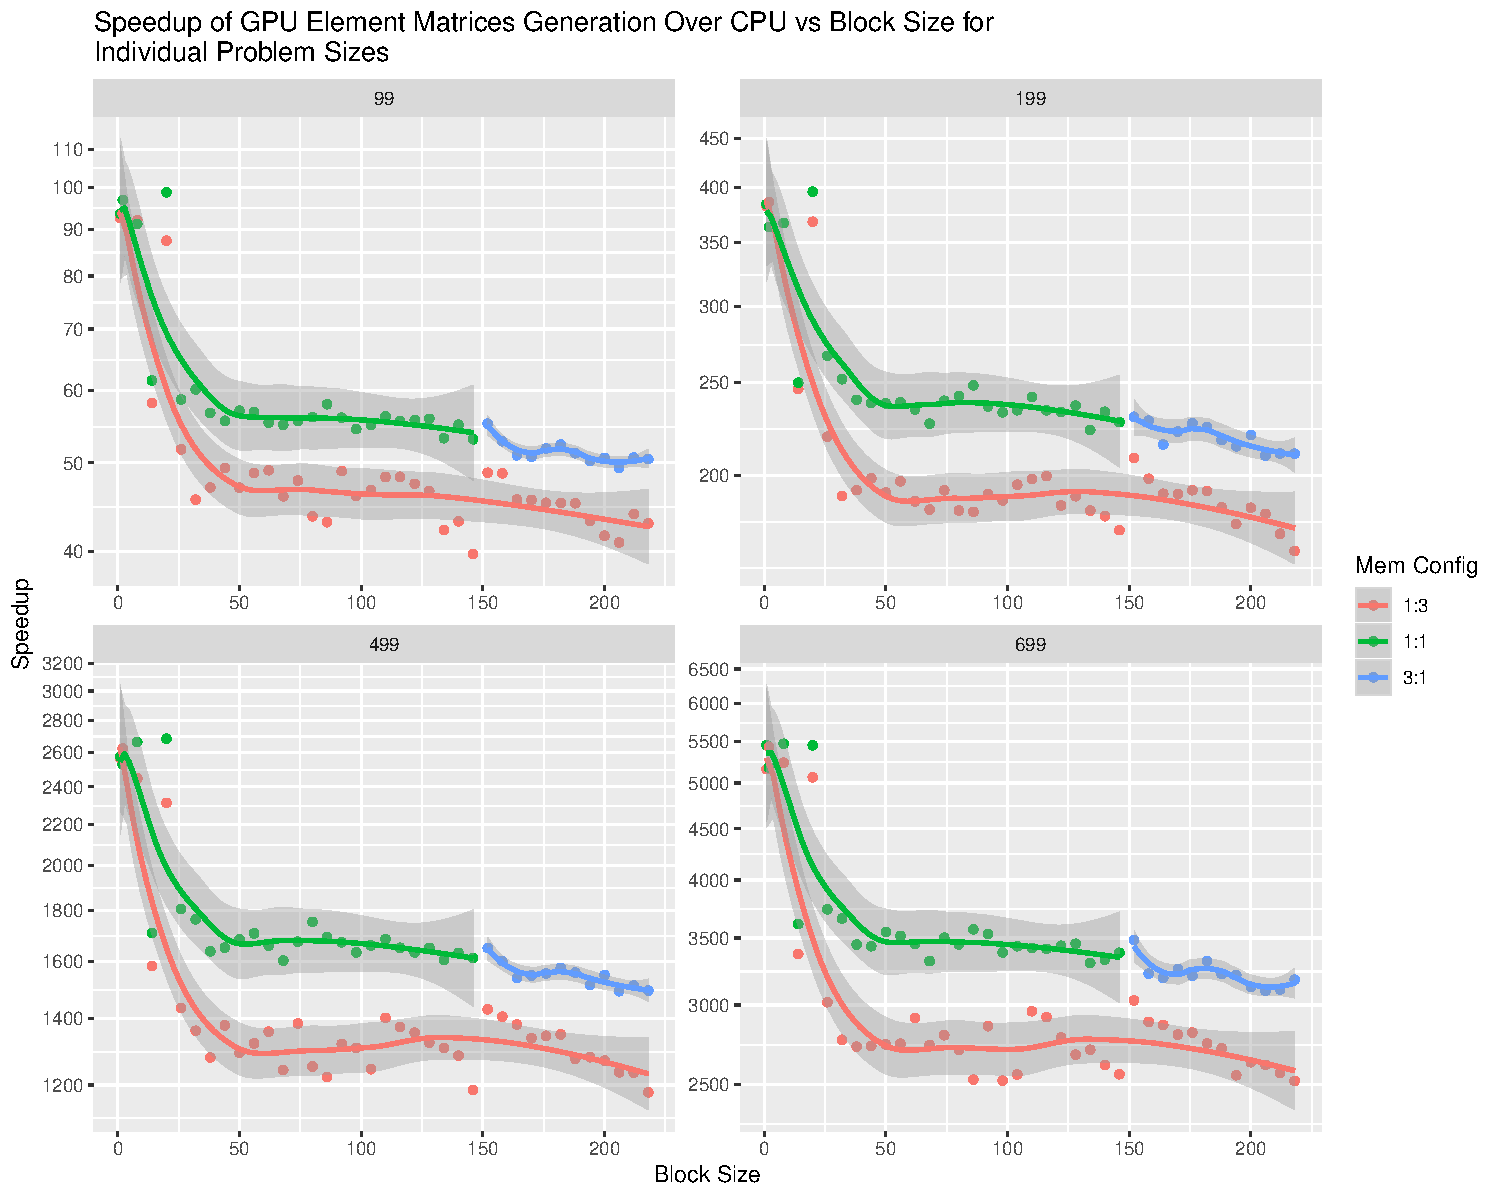
\includegraphics[width=0.9\linewidth]{Plots/elem_mats_dev_speedups_reconfig}
	\caption{CAPTION}
	\label{fig:elems_reconfig}
\end{figure}

\subsubsection{Global Stiffness Matrix \& Stress Vector Assembly}

\begin{figure}
	\centering
	\begin{subfigure}{0.48\linewidth}
		\centering
		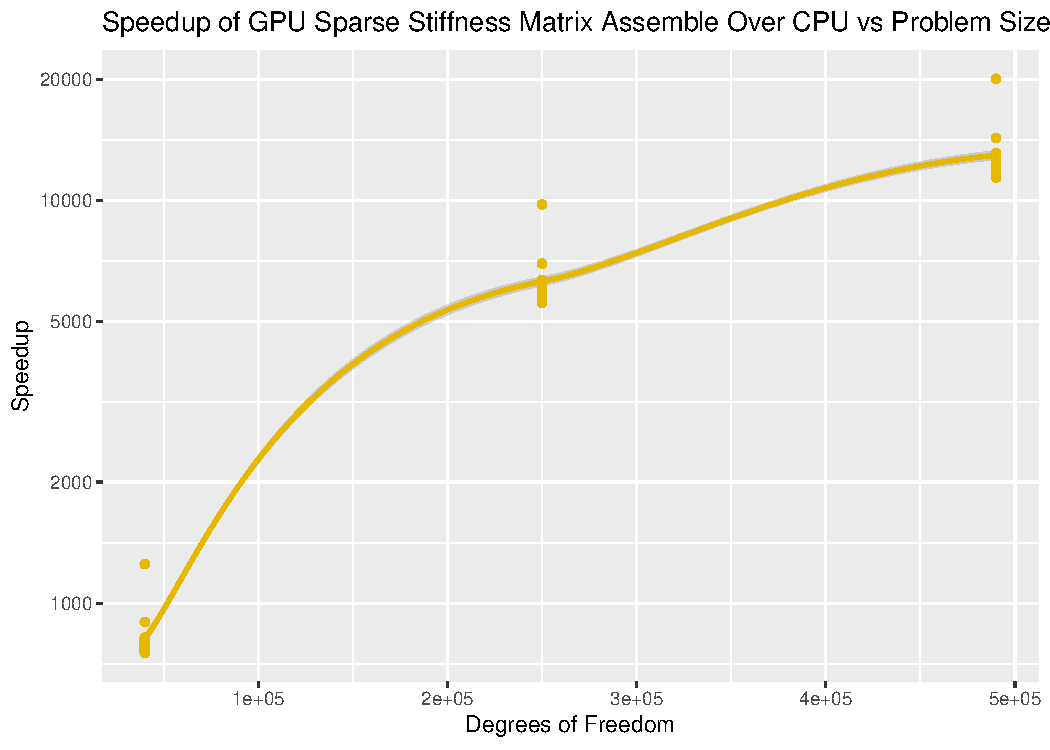
\includegraphics[width = \linewidth]{Plots/assem_dev_cpu_sparse_speedup_vs_n}
		\caption{Caption}
		\label{fig:assem_sparse_n}
	\end{subfigure}\hfill
	\begin{subfigure}{0.48\linewidth}
		\centering
		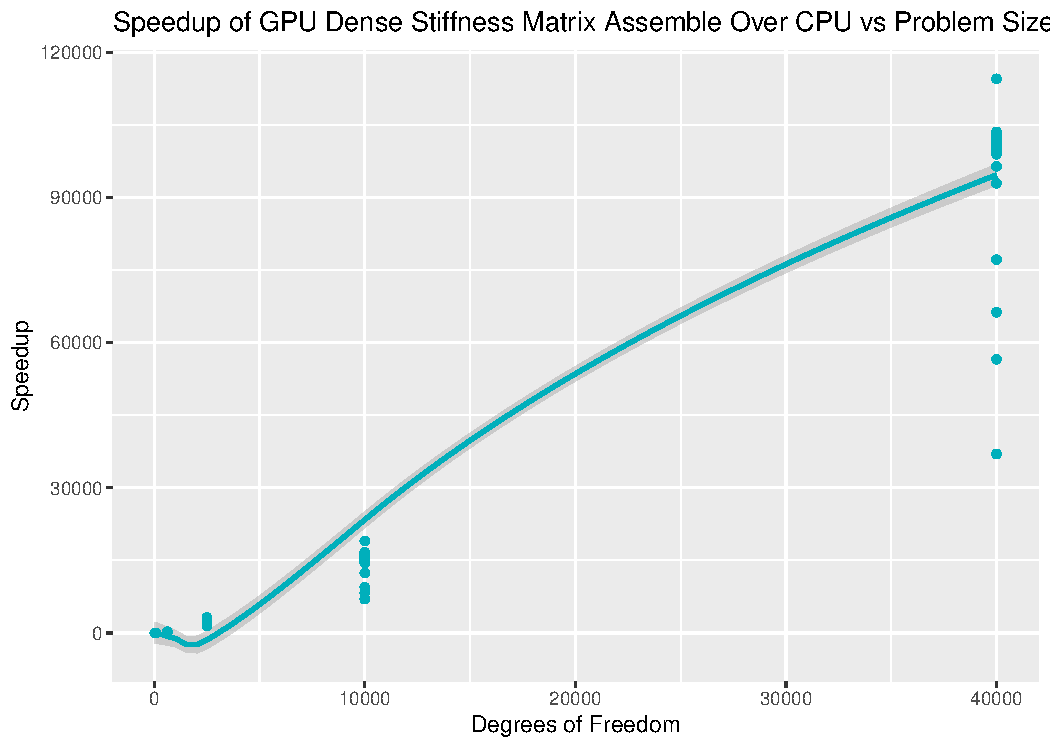
\includegraphics[width=\linewidth]{Plots/assem_dev_cpu_dense_speedup_vs_n}
		\caption{Caption}
		\label{fig:assem_dense_n}
	\end{subfigure}
	\caption{Speed-ups of GPU assembly of global stiffness matrix \& stress vector over serial code against problem size for CSR and dense matrices.}
	\label{fig:assem_su_n}
\end{figure}

The assembly of the global stiffness matrix and stress vector are another important point of optimisation in this study as it is another area which can provide huge amounts of parallelisation. Figure~\ref{fig:assem_su_n} shows the speed-ups seen for both sparse and dense variants of the device function, achieving even more impressive results than the element matrices generation. Both show massive speed-ups of $20,000\times$ and $100,000\times$, respectively. It might be an easy thought to assume that the sparse assembly would in fact be faster, but it as it turns out, to be slower than the dense assembly. Figure~\ref{fig:sparse_dense_assem} shows this fact. There are two contributing factors to this unexpected anomaly. The first being, there are far less variables, particularly pointers, needed in the dense assembly function and so there overflow of the, already-packed, registry memory is less of a factor. This can actually be seen in the initial spike and quick drop off in speed-up seen in Figure~\ref{fig:sparse_dense_assem}, before the thread registers overflow in the sparse function. The second, main contributing factor to this is the lack of coalescence and irregular memory access pattern of the CSR matrix. The algorithm requires jumping back and forward through three separate arrays to find the correct position in the matrix to perform an atomicAdd. This wouldn't particularly be an issue in the shared memory, but in global memory this will provide quite a slow down. The dense assembly on the other hand is more simple and is also sequential accessing so does not suffer from these bottlenecks. So it then begs the question, which should have already an obvious answer, is the trade off for a sparse solver better than a dense assembly?

\begin{figure}
	\centering
	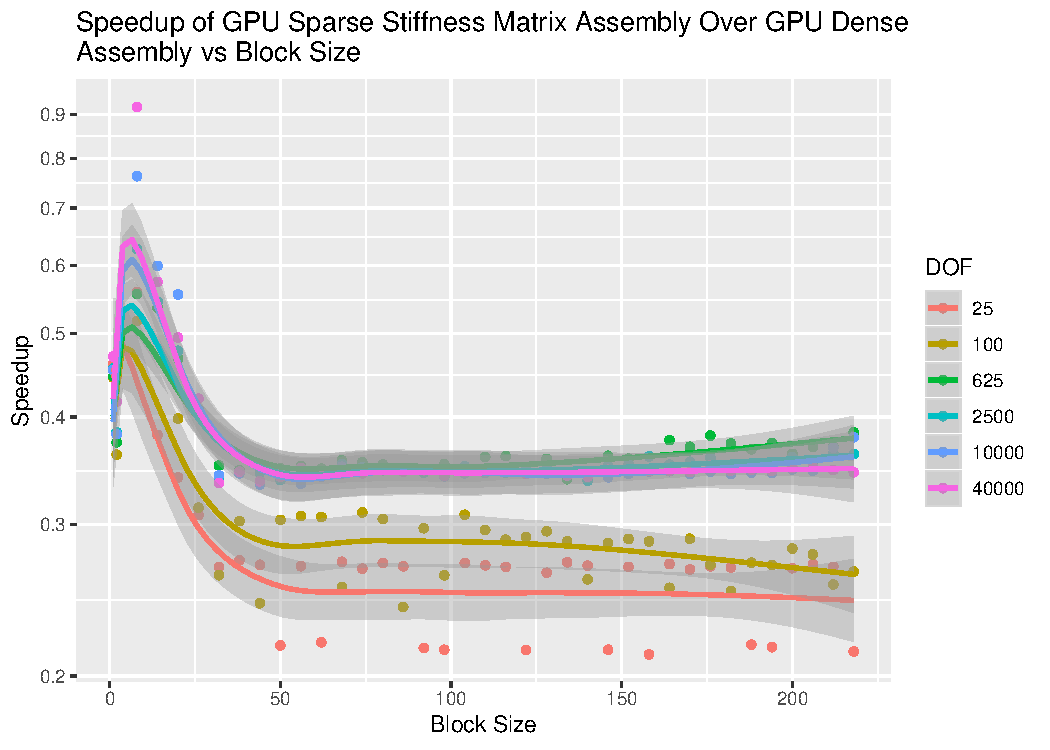
\includegraphics[width=0.55\linewidth]{Plots/assem_dev_gpu_sparse_dense_speedup_vs_b}
	\caption{Speed-ups of GPU sparse stiffness matrix assembly over dense versus block size.}
	\label{fig:sparse_dense_assem}
\end{figure}

Like in the element matrices, choice of block size does in fact matter - both for sparse and dense assembly. Figures~\ref{fig:assem_sparse_reconfig},~\ref{fig:assem_dense_reconfig} both show this. Like in the element matrices device functions, there isn't a clear indication from the plots of thread divergence causing a large effect but more so, oscillates in and around mutiples of 32 where the speed-ups increase. Again, also, reconfiguring the memory resulted in some positive results, barring overlaps in the smallest problem size. This could be down to the fact that all the threads in the block potentially not being used as the problem was not large enough.

\begin{figure}
	\centering
	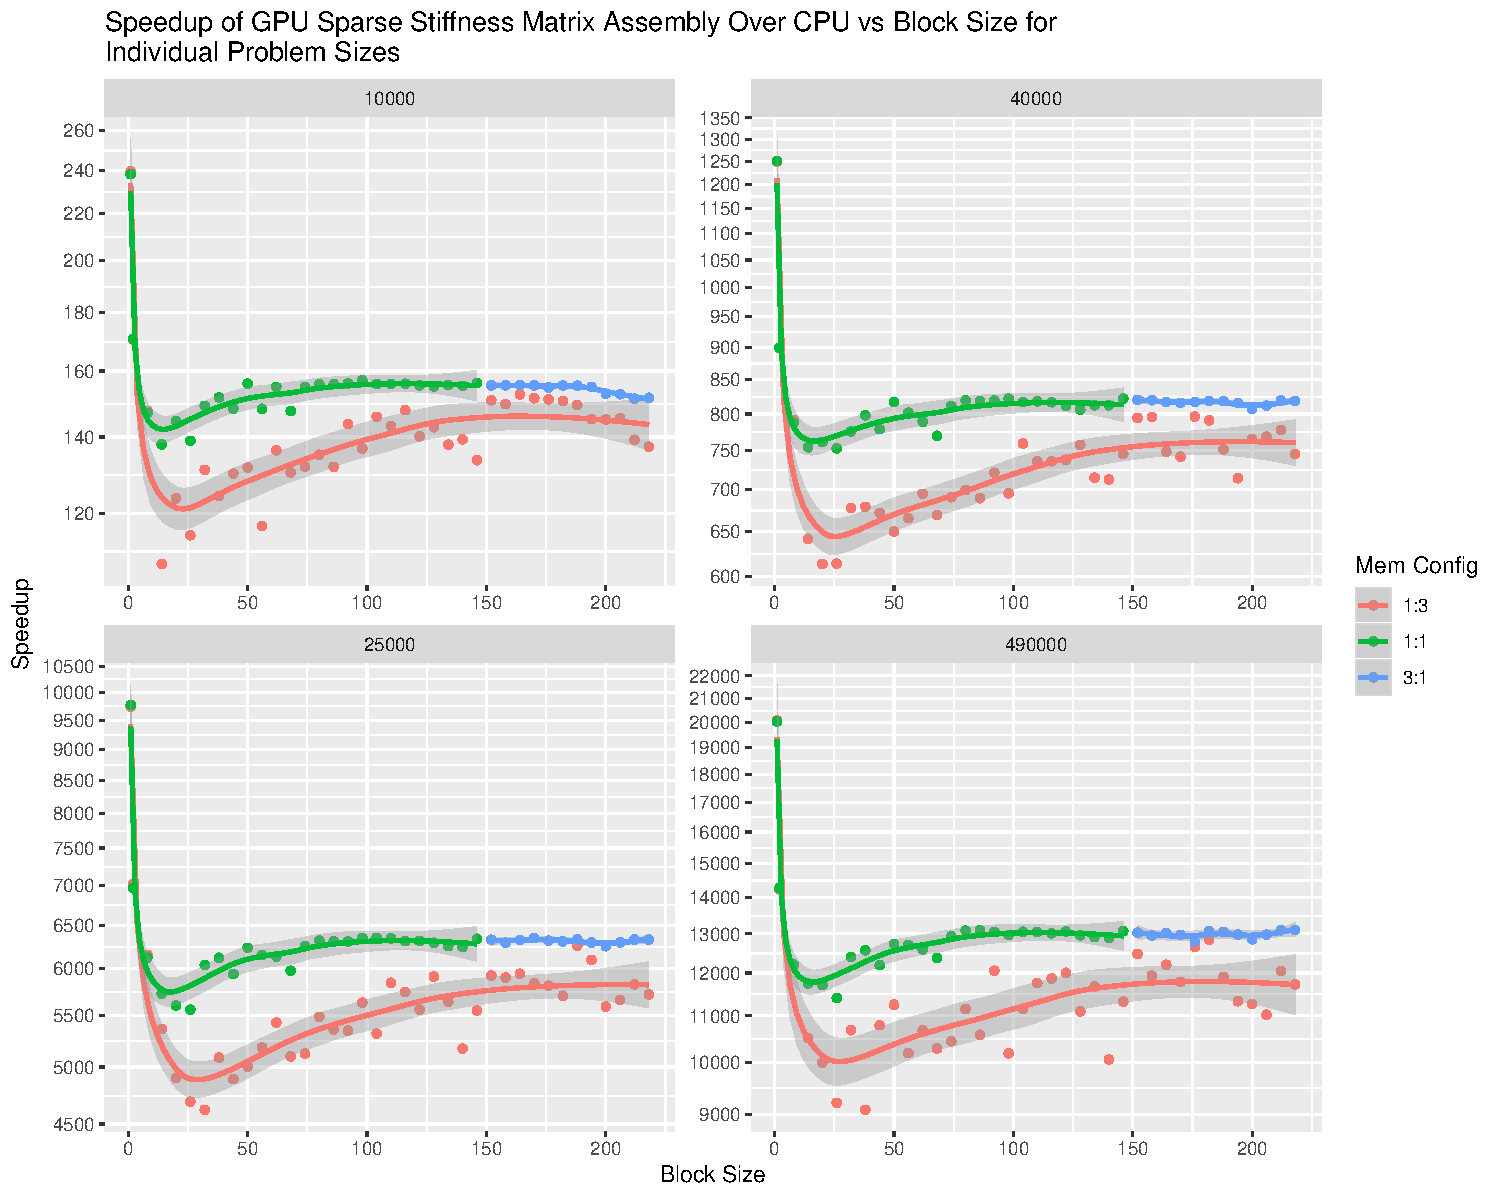
\includegraphics[width=0.9\linewidth]{Plots/assem_dev_sparse_speedups_reconfig}
	\caption{CAPTION}
	\label{fig:assem_sparse_reconfig}
\end{figure}

\begin{figure}
	\centering
	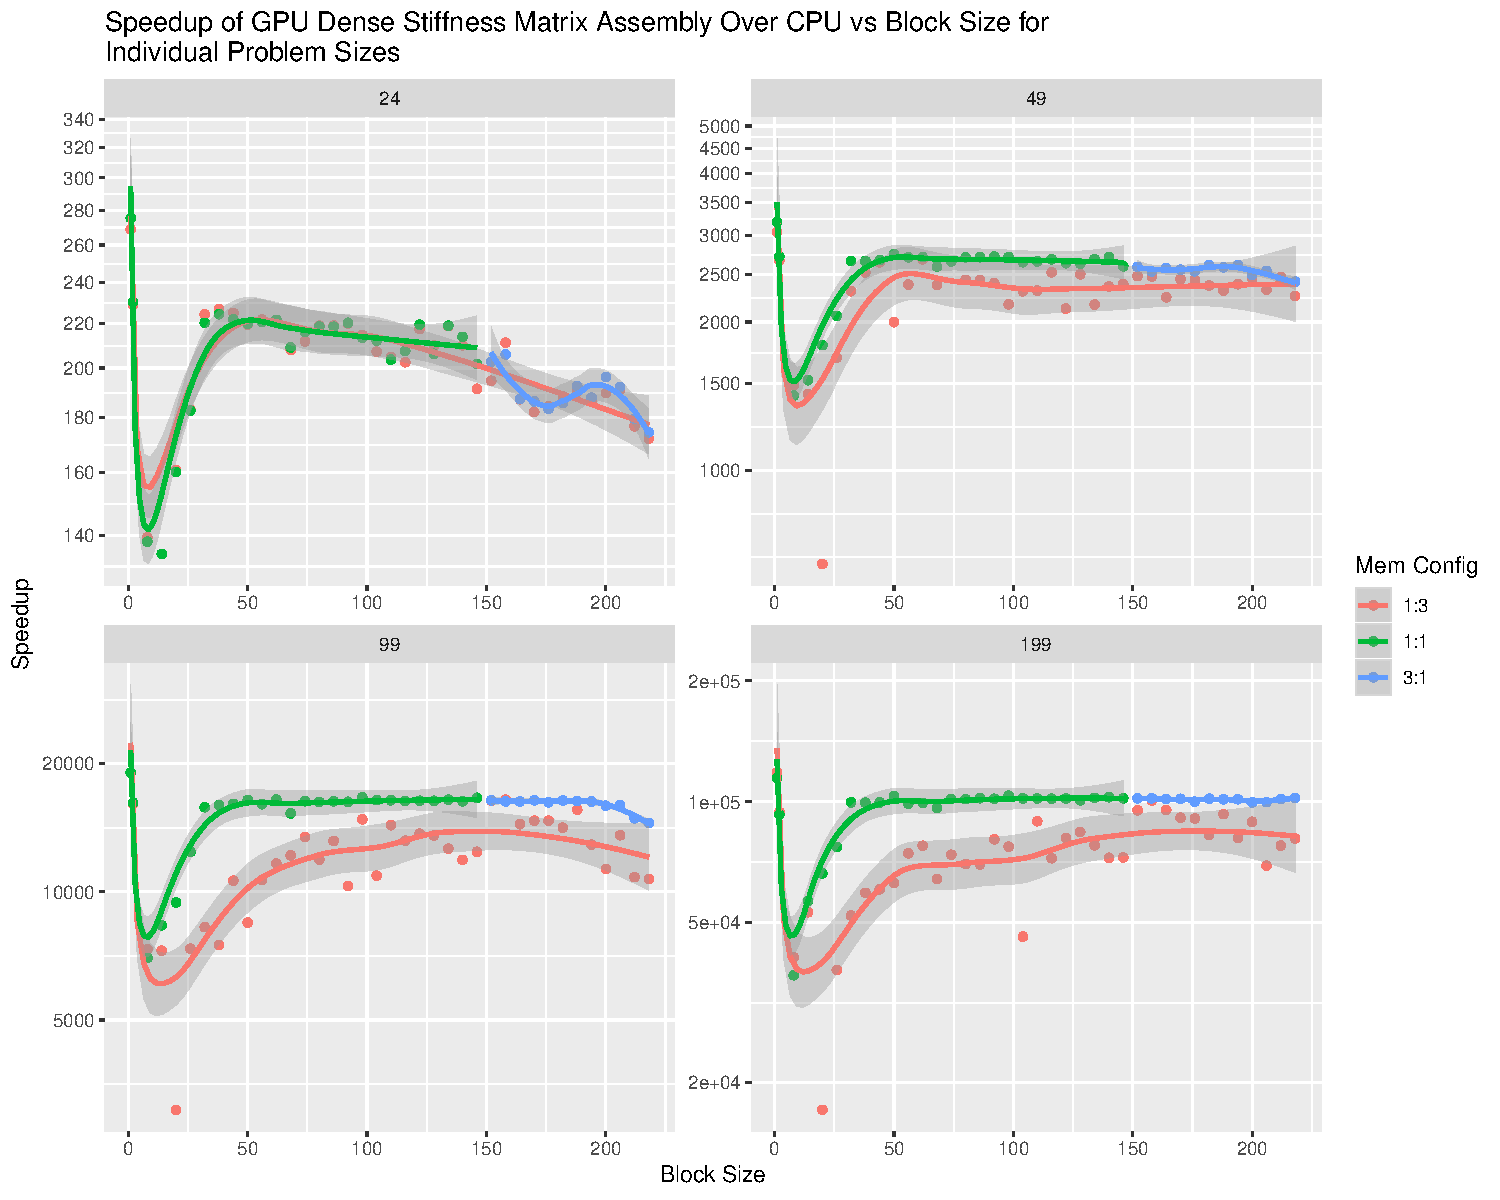
\includegraphics[width=0.9\linewidth]{Plots/assem_dev_dense_speedups_reconfig}
	\caption{CAPTION}
	\label{fig:assem_dense_reconfig}
\end{figure}


\subsubsection{Main Kernel Total}

\begin{figure}
	\centering
	\begin{subfigure}{0.48\linewidth}
		\centering
		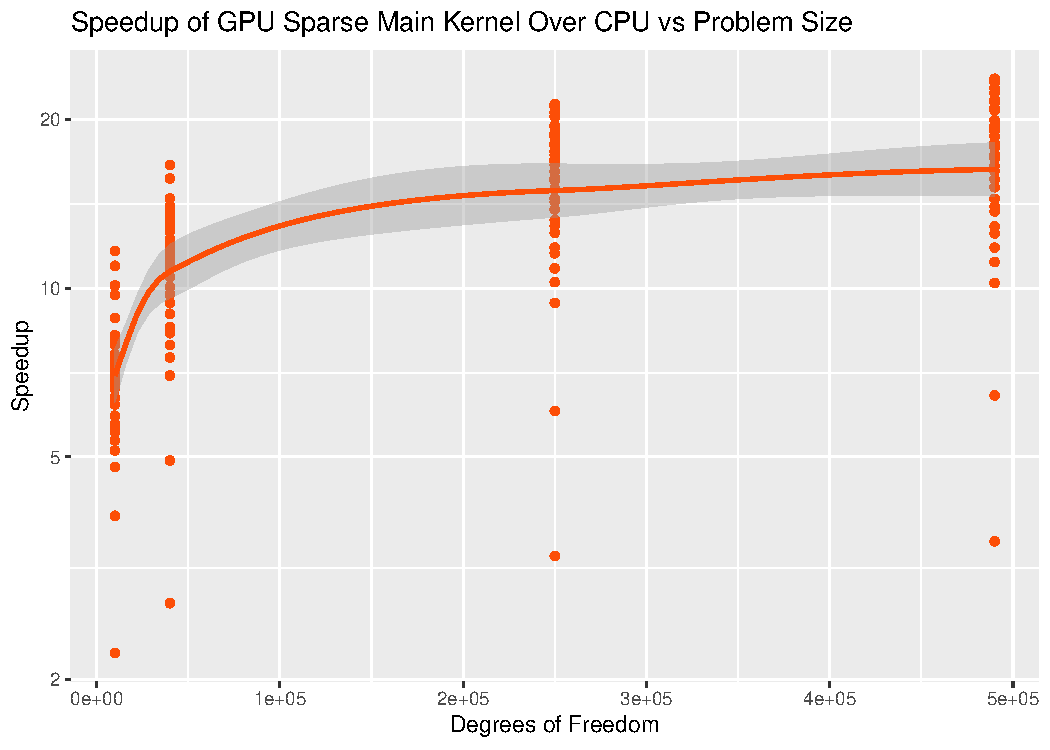
\includegraphics[width = \linewidth]{Plots/elems_p_assem_ker_cpu_sparse_speedup_vs_n}
		\caption{Caption}
		\label{fig:kern_sparse_n}
	\end{subfigure}\hfill
	\begin{subfigure}{0.48\linewidth}
		\centering
		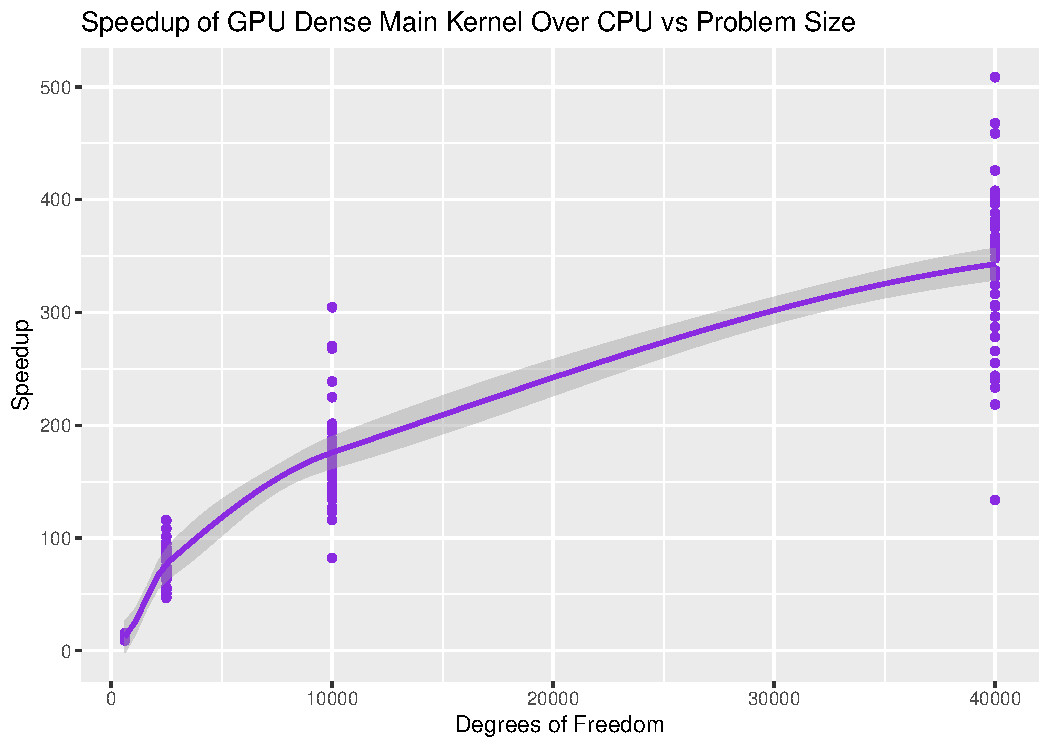
\includegraphics[width=\linewidth]{Plots/elems_p_assem_ker_cpu_dense_speedup_vs_n}
		\caption{Caption}
		\label{fig:kern_dense_n}
	\end{subfigure}
	\caption{Speed-ups of GPU main kernel over serial code against problem size for CSR and dense matrices.}
	\label{fig:kern_su_n}
\end{figure}

A downside to the timings for the two device functions is the lack of ability to use cudaEvents, which can only be used to time an kernel in its entirety. Instead, \texttt{clock64()} must to be utilised. This takes the clock ticks on each thread, which then must be written back to a global memory array, and then using cuBLAS, the max of this array calculated - giving the theoretical maximum time taken for the device function to finish. Unfortunately, in reality, that isn't how perfectly kernels and device functions run as other threads end up stalling while waiting for others and the kernel cannot complete until the al the threads are finished. This is a bottleneck of CUDA programming and unavoidable. For example, when taking the cudaEvents time for the entire kernel, the irregular memory access pattern of writing these times into global memory must be taken into account as all the threads cannot finish the kernel until the entire array of clock cycles has been populated.

With that being said, for a more realistic speed-up time, the entire kernel was timed and these times are illustrated in Figures~\ref{fig:kern_sparse_n},~\ref{fig:kern_sparse_n}. Even with the device timings being taken, the kernel still demonstrates faster execution times than in serial for both sparse and dense cases, reaching up to around $20\times$ and $300\times$, respectively. These times can be effectively taken as a minimum speed-up as removing the clock cycle evaluation will reduce these even further.

Overall then, considering that the only part of the entire process that was attempted to be parallelised took up around (PERCENTAGE) of the entire computation time, the amount of speed-ups achieved in that small portion proved quite substantial

\subsection{FEMSES}

\subsection{Comparison of GPU Architectures}